% ============================================================
%  RESUMEN EJECUTIVO -- SEGUNDA ENTREGA
%  Álgebra Lineal Aplicada
%  Péndulo invertido sobre un carro (tres configuraciones)
%  Universidad Nacional de Colombia -- Sede Medellín
%  Mismo formato que el informe técnico; máximo 5 páginas.
% ============================================================
\documentclass[11pt,letterpaper]{article}

% ── Idioma y codificación ───────────────────────────────────
\usepackage[utf8]{inputenc}
\usepackage[T1]{fontenc}
\usepackage[spanish,provide=*]{babel}

% ── Tipografía (Palatino, look de tesis) ────────────────────
\usepackage{mathpazo}
\usepackage{microtype}
\linespread{1.02}

% ── Geometría de página ─────────────────────────────────────
\usepackage[letterpaper,top=0.9in,bottom=0.9in,left=1in,right=1in]{geometry}

% ── Matemáticas ─────────────────────────────────────────────
\usepackage{amsmath,amssymb,mathtools,bm}

% ── Color, cajas, tablas, figuras ───────────────────────────
\usepackage{xcolor}
\definecolor{acento}{RGB}{31,59,107}
\definecolor{acento2}{RGB}{120,40,40}
\usepackage[most]{tcolorbox}
\usepackage{booktabs}
\usepackage{array}
\usepackage{graphicx}

% ── Títulos de sección ──────────────────────────────────────
\usepackage{titlesec}
\titleformat{\section}
  {\normalfont\large\bfseries\color{acento}}{\thesection}{0.7em}{}
\titleformat{\subsection}
  {\normalfont\normalsize\bfseries\color{acento!85!black}}{\thesubsection}{0.6em}{}
\titlespacing*{\section}{0pt}{1.0ex plus .7ex minus .2ex}{0.5ex plus .2ex}
\titlespacing*{\subsection}{0pt}{0.8ex plus .5ex minus .2ex}{0.4ex plus .2ex}

% ── Encabezado/pie ──────────────────────────────────────────
\usepackage{fancyhdr}
\pagestyle{fancy}\fancyhf{}
\renewcommand{\headrulewidth}{0.4pt}
\fancyhead[L]{\footnotesize\itshape Resumen ejecutivo (segunda entrega) --- Péndulo invertido}
\fancyhead[R]{\footnotesize\itshape Álgebra Lineal Aplicada}
\fancyfoot[C]{\thepage}

% ── Listas y enlaces ────────────────────────────────────────
\usepackage{enumitem}
\setlist{itemsep=1.5pt,topsep=2pt}
\usepackage[colorlinks=true,linkcolor=acento,citecolor=acento2,urlcolor=acento]{hyperref}
\usepackage{cleveref}

% ── Cajas ───────────────────────────────────────────────────
\newtcolorbox{clave}[1][]{colback=acento!4,colframe=acento!55!black,
  boxrule=0.6pt,arc=2pt,left=6pt,right=6pt,top=5pt,bottom=5pt,#1}

% ── Operadores y atajos ─────────────────────────────────────
\DeclareMathOperator{\rank}{rango}
\DeclareMathOperator{\diag}{diag}
\newcommand{\R}{\mathbb{R}}
\newcommand{\C}{\mathbb{C}}
\newcommand{\calC}{\mathcal{C}}
\newcommand{\calO}{\mathcal{O}}
\newcommand{\xv}{\bm{x}}
\newcommand{\uv}{\bm{u}}
\newcommand{\ev}{\bm{e}}

\crefname{table}{tabla}{tablas}\Crefname{table}{Tabla}{Tablas}
\crefname{figure}{figura}{figuras}\Crefname{figure}{Figura}{Figuras}
\addto\captionsspanish{\renewcommand{\tablename}{Tabla}}

% Figuras: las propias del informe técnico de esta entrega y los mapas del atlas.
\graphicspath{{../informe_tecnico/figs/}{../atlas/figs/}}

% ============================================================
\begin{document}

% ── Cabecera ────────────────────────────────────────────────
\begin{center}
    {\footnotesize\bfseries\color{acento2} RESUMEN EJECUTIVO --- SEGUNDA ENTREGA}\\[0.4em]
    {\LARGE\bfseries El Límite No Es Teórico, Es Numérico}\\[0.6em]
    {\normalsize Mateo Bedoya Rojas \quad\textbullet\quad Camilo Alejandro Patiño Osorio \quad\textbullet\quad Santiago Uribe Echavarría}\\[0.3em]
    {\footnotesize Facultad de Ciencias, Universidad Nacional de Colombia, Sede Medellín}
\end{center}
\vspace{0.2em}
\hrule height 0.6pt
\vspace{0.8em}

\noindent
\begin{clave}
\small
\textbf{Propósito.} Este documento resume de forma ejecutiva la segunda entrega
del proyecto y sirve de guía para recorrerla. Las deducciones, demostraciones y
tablas completas están en el \emph{informe técnico de esta
entrega}~\cite{tecnico2}, al que se remite en cada sección. La primera entrega
se documenta por separado~\cite{tecnico1}.
\end{clave}

% ============================================================
\section{Punto de partida y objetivo}

La primera entrega demostró que el péndulo invertido, en sus configuraciones
\emph{simple} ($\R^4$) y \emph{doble} ($\R^6$), es inestable pero controlable y
observable, y lo estabilizó con realimentación de estado $\uv=-K\xv$ diseñada
por LQR y por asignación de polos. El resultado era correcto, pero dejaba cinco
huecos que un lector crítico podía señalar. Esta entrega los ataca:

\begin{enumerate}
  \item La observabilidad se \emph{analizaba} y no se \emph{usaba}: se controlaba
  con el estado completo, que en la práctica no se mide.
  \item No había noción de \emph{límite de validez}: se sabía que el controlador
  funciona, no hasta dónde.
  \item El criterio de rango de Kalman es \emph{binario y frágil}, y eso no se
  decía.
  \item No había \emph{pruebas automatizadas} que blindaran los resultados.
  \item Con solo \emph{dos} configuraciones, la afirmación ``el método escala''
  es anecdótica.
\end{enumerate}

\noindent\emph{Detalle: informe técnico~\cite{tecnico2}, Sección~1.}

% ============================================================
\section{Qué se hizo}

\textbf{Una familia en lugar de tres problemas.} Se reformuló el modelo para $N$
eslabones arbitrarios. Las configuraciones I y II resultan casos particulares
($N=1$ con barra uniforme, $N=2$ con masas puntuales) y la nueva
\textbf{Configuración III} ---el péndulo triple, estado en $\R^8$, cuatro grados
de libertad y un solo actuador--- es el siguiente término. Como los modelos
antiguos se conservaron intactos, la coincidencia entre ambos es una prueba
entre \emph{implementaciones independientes}, no un acto de fe: la discrepancia
máxima medida es $5.3\times10^{-15}$ para $N=1$ y \emph{exactamente cero} para
$N=2$.

\textbf{Una métrica que reemplaza al rango.} Se introdujo el \emph{margen de
Popov--Belevitch--Hautus}~\cite{chen1999}, que sustituye el rango por el menor
valor singular de
$[A-\lambda I\mid B]$. Por el teorema de Eckart--Young~\cite{eckart1936} esa cantidad es
exactamente la distancia en norma 2 a perder la controlabilidad: mide
\emph{cuánto habría que perturbar el sistema} para volverlo incontrolable.

\textbf{Un atlas de operabilidad.} Se barrió el espacio de parámetros integrando
el modelo \emph{no lineal} con saturación en cada punto, separando la
imposibilidad \emph{estructural} (propiedad del sistema) de la \emph{práctica}
(propiedad de la implementación).

\textbf{Un observador de estado.} Se cerró el hueco 1 con un observador de
Luenberger~\cite{ogata2010} diseñado por \emph{dualidad de Kalman}, que
reutiliza la misma ecuación de Riccati del controlador sin escribir ningún
algoritmo nuevo.

\textbf{618 pruebas de regresión}, que contrastan los jacobianos analíticos
contra diferenciación automática y reproducen cada cifra publicada.

\noindent\emph{Detalle: informe técnico~\cite{tecnico2}, Secciones~2 a~8.}

% ============================================================
\section{Resultados}

\begin{table}[htbp]
  \centering\small
  \caption{Las tres configuraciones con sus parámetros por defecto.
  $\operatorname{cond}\calC$ es el número de condición de la matriz de Kalman y
  $h_{\max}$ el mayor período de muestreo que conserva la estabilidad en tiempo
  discreto.}
  \label{tab:exec2}
  \begin{tabular}{@{}lcccccc@{}}
    \toprule
    \textbf{Config.} & $n$ & \textbf{inest.} & $\lambda_{\max}$ [s$^{-1}$] & $\operatorname{cond}\calC$ & $\|K\|_2$ & $h_{\max}$ [ms]\\
    \midrule
    Simple & 4 & 1 & 4.21  & $3.6\times10^{1}$ & 47.0   & 197.4\\
    Doble  & 6 & 2 & 8.57  & $1.6\times10^{4}$ & 300.5  & 77.3\\
    Triple & 8 & 3 & 18.06 & $2.2\times10^{8}$ & 1176.0 & 32.0\\
    \bottomrule
  \end{tabular}
\end{table}

\textbf{La Configuración III se controla.} Espectro de lazo abierto con
\emph{tres} modos inestables, el dominante en $+18.06$~s$^{-1}$ ---el sistema se
desploma cuatro veces más rápido que el simple---, rangos $8/8$ y estabilización
completa en 1.88~s con un pico de fuerza de 7.29~N.

\textbf{El álgebra escala, el condicionamiento no.} Éste es el resultado
central. El criterio de rango sigue dando la respuesta correcta para las tres
configuraciones, pero el condicionamiento~\cite{golub2013} de la matriz de
Kalman crece unos
cuatro órdenes de magnitud por eslabón: con cinco eslabones llega a
$3.3\times10^{16}$, siete veces por encima de $1/\varepsilon_{\text{máq}}$, y el
rango numérico pasa a ser \emph{ruido} aunque el sistema siga siendo controlable
en aritmética exacta. El margen PBH, en cambio, decae suavemente ---poco más de
dos órdenes en el mismo rango--- y sigue siendo utilizable.

\begin{figure}[htbp]
  \centering
  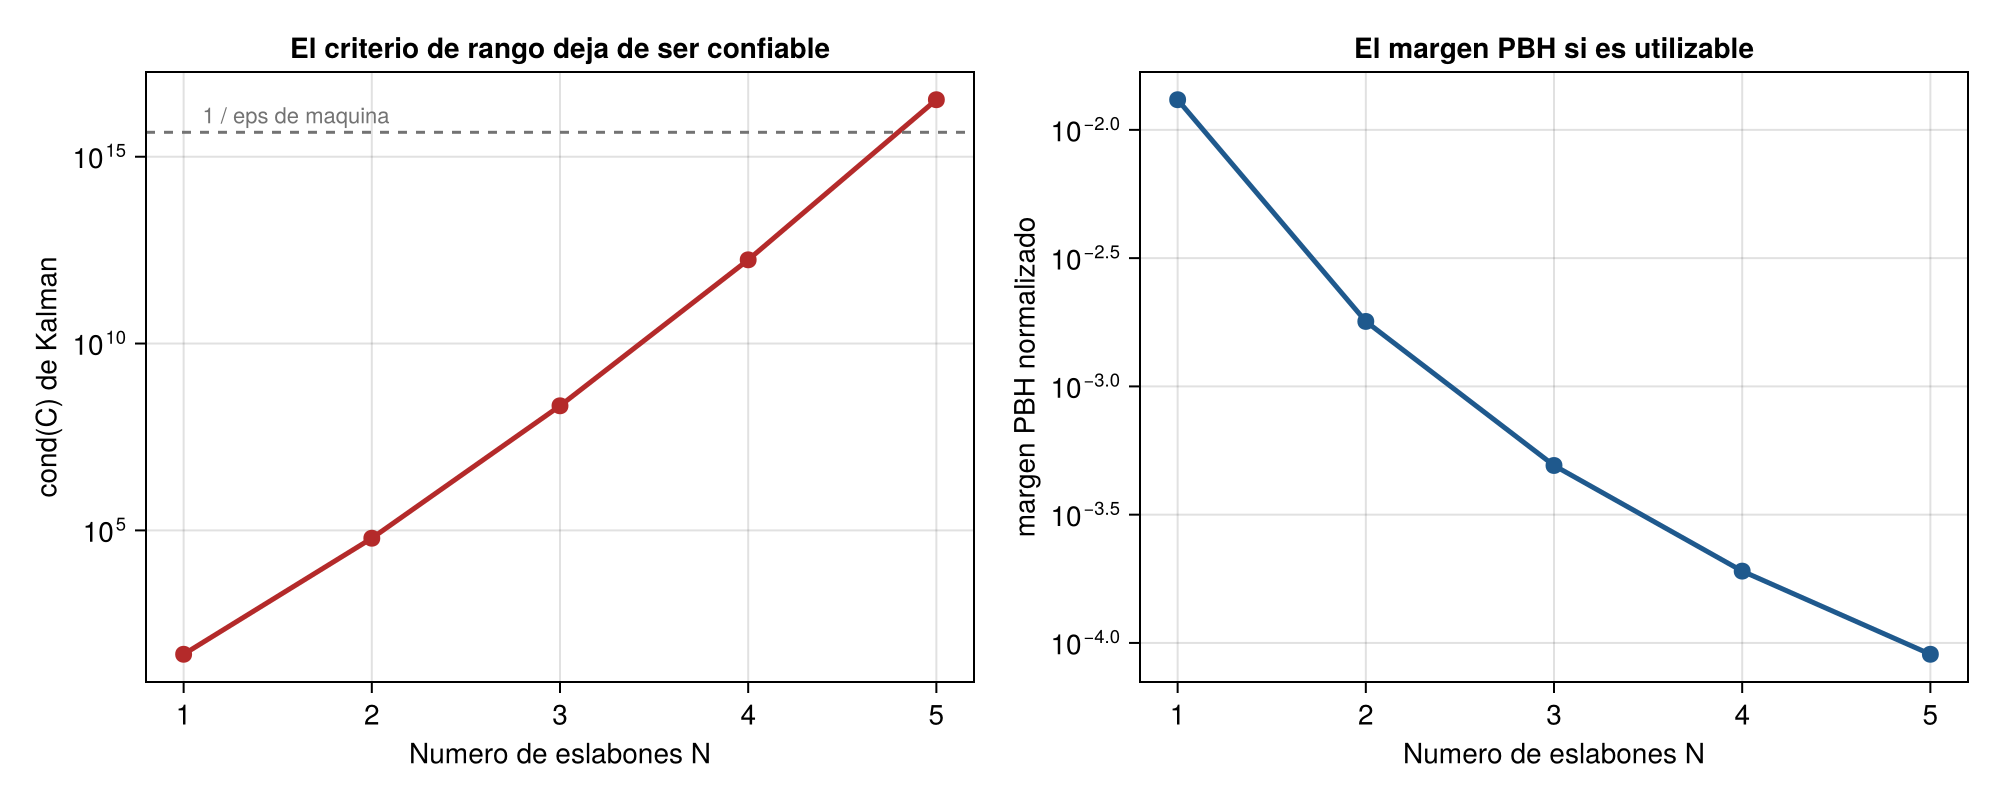
\includegraphics[width=\linewidth]{degradacion_N.png}
  \caption{Izquierda: el condicionamiento de $\calC$ cruza el umbral de la
  precisión de máquina. Derecha: el margen PBH decae suavemente. El teorema
  sigue siendo cierto; el algoritmo que lo implementa deja de serlo.}
  \label{fig:exec2deg}
\end{figure}

\textbf{Hay una configuración óptima, y no está en los extremos.} El margen PBH
tiene un \emph{máximo interior} en una masa de carro de $0.126$~kg: un carro muy
pesado se mueve poco ante la misma fuerza y pierde autoridad de control, uno muy
liviano degrada el acoplamiento con los eslabones. Distintas métricas señalan
óptimos distintos, lo cual es en sí mismo un resultado: no existe ``la'' mejor
configuración sin decir antes qué se optimiza.

\textbf{La frontera de operabilidad, y dónde falla la garantía.} La cota
elipsoidal $c^\star=u_{\max}^2/(KP^{-1}K^\top)$ ---una garantía dura obtenida
con Cauchy--Schwarz sobre la forma cuadrática de Lyapunov~\cite{olver2018}---
queda por dentro de la frontera real mientras la
saturación sea la restricción activa, pero la cruza a partir de $u_{\max}=85$~N.
La razón es que $c^\star$ solo certifica no saturación más convergencia
\emph{lineal}, y más allá de ese punto lo que limita es la no linealidad.

\begin{figure}[htbp]
  \centering
  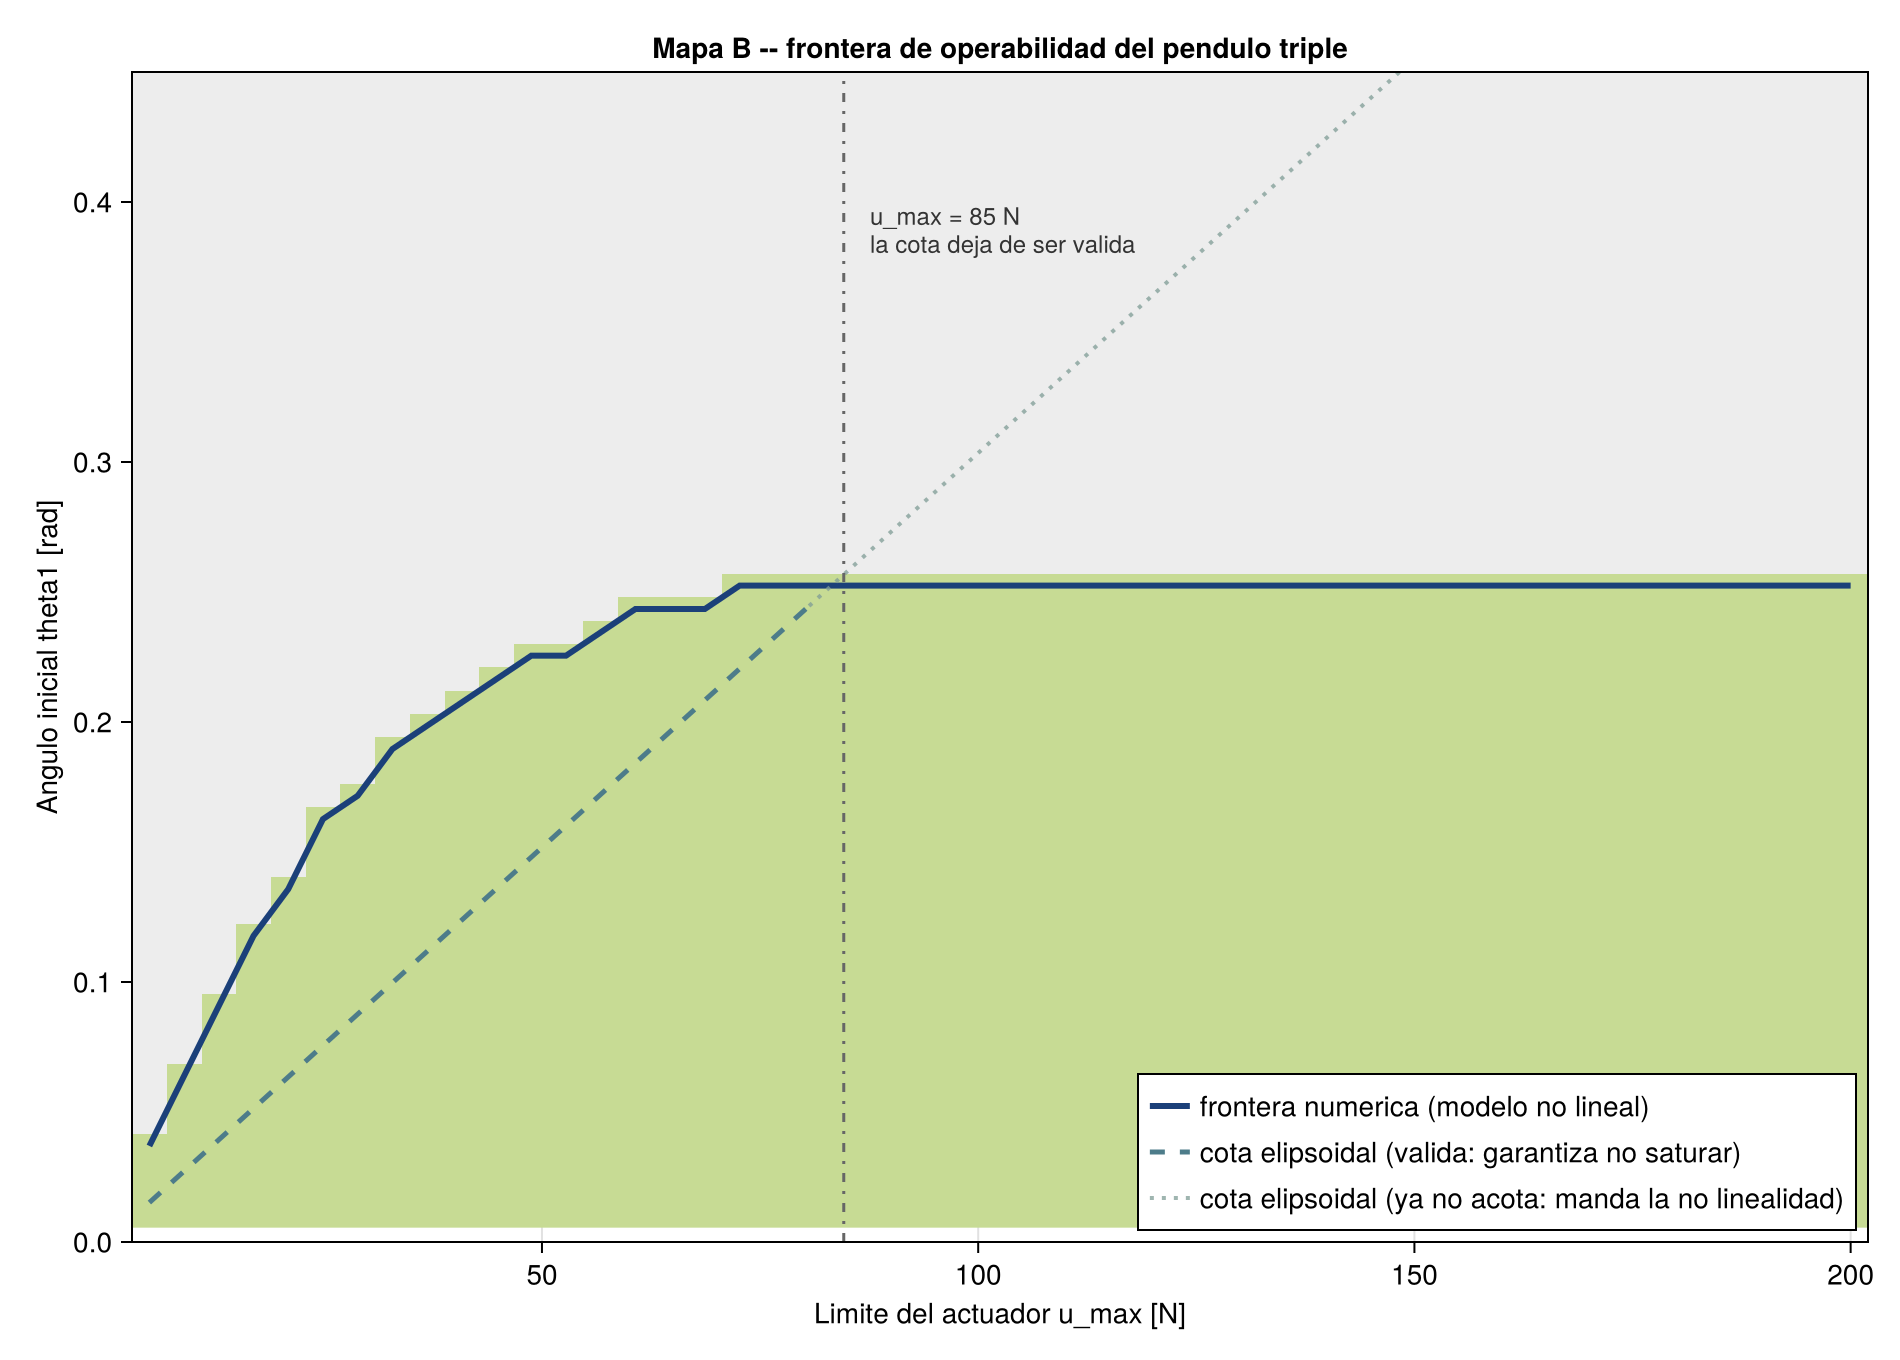
\includegraphics[width=0.86\linewidth]{atlas_b.png}
  \caption{Frontera de operabilidad del péndulo triple. La zona clara es donde
  el controlador recupera. La cota analítica es válida hasta el punto marcado;
  más allá promete más de lo que el sistema no lineal cumple.}
  \label{fig:exec2atlas}
\end{figure}

\textbf{Basta un sensor, pero apenas.} De los 15 subconjuntos posibles de
sensores del péndulo triple, \emph{todos} los que incluyen la posición del carro
son observables y \emph{ninguno} que la excluya lo es: midiendo solo ángulos, la
posición absoluta del carro es inobservable porque la dinámica angular es
invariante a trasladarlo. El juego mínimo es un único sensor ---la posición---
suficiente para reconstruir los ocho estados; pero con un margen dos órdenes
peor que el del juego completo. \emph{Observable no es lo mismo que
practicable}, distinción que un criterio binario de rango no puede expresar.

\noindent\emph{Tablas y figuras completas: informe técnico~\cite{tecnico2},
Secciones~3 a~7.}

% ============================================================
\section{Honestidad sobre el alcance}

Varias predicciones del plan de trabajo resultaron incorrectas al medirlas, y se
registran como parte del resultado:

\begin{itemize}
  \item El actuador de 150~N no hacía falta por la razón que se creía: con la
  condición inicial nominal los términos de $K$ se cancelan y el pico real es de
  7.29~N, no de los $\approx46$~N estimados.
  \item La cota elipsoidal no queda por dentro de la frontera en todo el rango,
  sino solo mientras la saturación mande.
  \item La restricción práctica activa \emph{cambia} con la configuración: en el
  péndulo simple el límite lo pone el riel, no el motor ni la no linealidad.
  \item Cuatro órdenes de magnitud en el peso $R$ del control mueven $\|K\|$
  apenas un factor 2: la planta es tan inestable que cualquier controlador que
  la estabilice necesita ganancia grande, y ajustar $R$ compra muy poco.
  \item \textbf{El observador no sale gratis.} El principio de separación
  garantiza estabilidad del sistema \emph{lineal}, pero sobre el modelo no
  lineal la región de atracción se encoge a entre la mitad y la cuarta parte,
  porque durante los primeros instantes el controlador actúa sobre una
  estimación equivocada. La condición inicial nominal de este trabajo se
  recupera con estado completo y \emph{no} se recupera con observador.
\end{itemize}

Lo que queda \emph{propuesto} y no medido: la capa no lineal de la región de
atracción (acotar el residuo de la linealización para obtener una garantía
rigurosa también fuera del régimen lineal) y el rediseño del LQR directamente en
tiempo discreto.

% ============================================================
\section{Conclusión}

El mismo puñado de conceptos de álgebra lineal ---exponencial matricial,
análisis espectral, teoría del rango, valores singulares y dualidad--- basta
para modelar, analizar, controlar y \emph{estimar} un sistema dinámico
subactuado de creciente complejidad. Pero al escalar aparece un límite que no es
teórico sino numérico: los criterios binarios de rango dejan de ser confiables
mucho antes de que la teoría deje de aplicar. La respuesta no es cambiar de
teoría sino de herramienta, y la herramienta adecuada ---el menor valor singular,
vía Eckart--Young--- vive en el mismo cuerpo de álgebra lineal
aplicada~\cite{olver2018,boyd2018}. Esa es la lección de esta entrega.

% ============================================================
% Ordenadas alfabéticamente por apellido del primer autor; entre obras del mismo
% autor, por título.
\begin{thebibliography}{9}
\small
\bibitem{tecnico1}
M.~Bedoya, C.~Patiño y S.~Uribe, \emph{Análisis del Péndulo Invertido sobre un
Carro mediante Álgebra Lineal Aplicada --- Informe Técnico, primera entrega}.
Universidad Nacional de Colombia, Sede Medellín, 2026.

\bibitem{tecnico2}
M.~Bedoya, C.~Patiño y S.~Uribe, \emph{El Límite No Es Teórico, Es Numérico ---
Informe Técnico, segunda entrega}. Universidad Nacional de Colombia, Sede
Medellín, 2026.

\bibitem{boyd2018}
S.~Boyd y L.~Vandenberghe, \emph{Introduction to Applied Linear Algebra:
Vectors, Matrices, and Least Squares}. Cambridge: Cambridge University Press,
2018.

\bibitem{chen1999}
C.-T.~Chen, \emph{Linear System Theory and Design}, 3.\textsuperscript{a} ed.
New York: Oxford University Press, 1999.

\bibitem{eckart1936}
C.~Eckart y G.~Young, ``The approximation of one matrix by another of lower
rank'', \emph{Psychometrika}, vol.~1, n.\textsuperscript{o}~3, pp.~211--218, 1936.

\bibitem{golub2013}
G.~H.~Golub y C.~F.~Van Loan, \emph{Matrix Computations},
4.\textsuperscript{a} ed. Baltimore: Johns Hopkins University Press, 2013.

\bibitem{ogata2010}
K.~Ogata, \emph{Modern Control Engineering}, 5.\textsuperscript{a} ed.
Upper Saddle River, NJ: Prentice Hall, 2010.

\bibitem{olver2018}
P.~J.~Olver y C.~Shakiban, \emph{Applied Linear Algebra},
2.\textsuperscript{a} ed. Cham: Springer, 2018.

\end{thebibliography}

\end{document}
